\begin{minipage}{0.62\linewidth}
    On fixe un ressort horizontal, de spires non jointives, de masse négligeable
    et de raideur $K$, à une bille (Fig.~\ref{fig:solide_ressort_bille}).

    Pour étudier le mouvement du centre d'inertie $G$ de la bille, on choisit un
    repère $(O,\ex)$ tel que l'origine $O$ coïncide avec la position de $G$ à
    l'équilibre ($x_G=0$), lorsque le ressort n'est pas déformé.

    On écarte la bille de sa position d'équilibre, puis on la libère sans
    vitesse initiale à l'instant $t_0=0$. On considère que la trajectoire de $G$
    est rectiligne.

    La Fig.~\ref{fig:2bac_svt_national_arabe_2011_normale_phys_ex3_2} représente
    le graphe de l'élongation $x_G=f(t)$ du mouvement de $G$.

    % \begin{donnees}
    %     \begin{itemize}
    %         \item $m=\qty{0.05}{\kg}$~; les frottements sont négligeables.
    %     \end{itemize}
    % \end{donnees}

    \textbf{\textsc{Données~:}}
    $m=\qty{0.05}{\kg}$~; les frottements sont négligeables.

    \begin{enumerate}[series=x]
        \item En appliquant la deuxième loi de Newton, établir l'équation
              différentielle vérifiée par l'abscisse $x_G$ du point
              $G$.~\textbf{(1,25pt)}

        \item La solution de l'équation différentielle s'écrit sous la forme~:
              $x_G(t)=X_m \cos\left(\frac{2\pi}{T_0}t+\varphi\right)$

              \begin{enumerate}[series=y]
                  \item Déterminer graphiquement les valeurs
                        de~:~\textbf{(1,5pt)}
                        \begin{itemize}
                            \item l'amplitude du mouvement $X_m$~;
                            \item la période propre de l'oscillateur $T_0$~;
                            \item la phase à l'origine $\varphi$, à l'instant
                                  $t_0=0$.
                        \end{itemize}
              \end{enumerate}
    \end{enumerate}
\end{minipage}
\hfill
\begin{minipage}{0.36\linewidth}
    \begin{figure}[H]
        \centering
        \input{figures/solide_ressort_bille}
        \caption{}
        \label{fig:solide_ressort_bille}
    \end{figure}
    \begin{figure}[H]
        \centering
        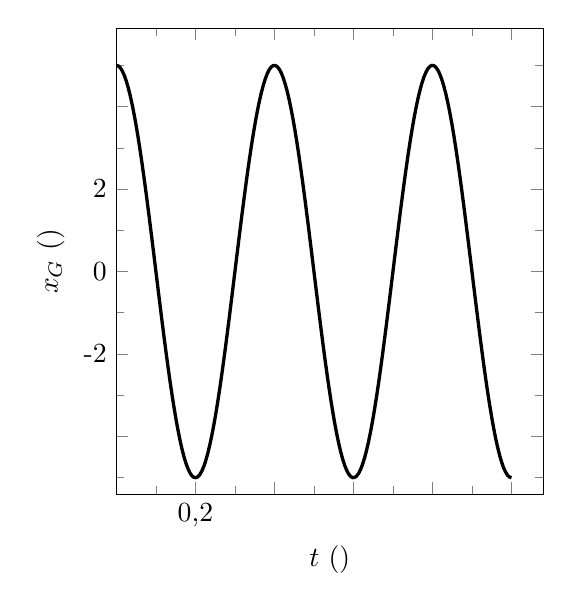
\begin{tikzpicture}
            \def\Xm{5}
            \def\T{0.4}
            \pgfmathpi\let\pi=\pgfmathresult
            \begin{axis}[
                    xmin=0,xmax=2.7*\T,
                    ymin=-5.4,ymax=5.9,
                    width=7cm,height=7.5cm,
                    trig format plots=rad,
                    xtick distance=0.2, ytick distance=2,
                    xticklabels={,,{0,2}}, yticklabels={,,-2,0,2},
                    xlabel=$t~(\unit{\second})$, ylabel=$x_{G}~(\unit{\cm})$,
                    minor tick num=1,
                ]
                \addplot[domain=0:2.5*\T,samples=200,very thick]
                    {\Xm*cos(2*pi/\T*x)};
            \end{axis}
        \end{tikzpicture}
        \caption{}
        \label{fig:2bac_svt_national_arabe_2011_normale_phys_ex3_2}
    \end{figure}
\end{minipage}

\begin{enumerate}[resume=x]
    \item[]
          \begin{enumerate}[resume=y]
              \item Calculer la valeur de la raideur $K$ du
                    ressort.~\textbf{(1pt)}
              \item Écrire l'expression de la vitesse $\dot{x}_G(t)$ du point
                    $G$.~\textbf{(1pt)}
              \item Déduire la valeur de $\dot{x}_G$ lors du premier passage de
                    la bille par sa position d'équilibre.~\textbf{(0,5pt)}
              \item Calculer la valeur de l'accélération $\ddot{x}_G$ du point
                    $G$ à l'instant~: $t=\frac{T_0}{2}$.~\textbf{(0,5pt)}
          \end{enumerate}
\end{enumerate}
